\documentclass[]{beamer}
% Class options include: notes, notesonly, handout, trans,
%                        hidesubsections, shadesubsections,
%                        inrow, blue, red, grey, brown

% Theme for beamer presentation.
\usepackage{beamerthemesplit} 



%%%%%%%%%%%%%%%%%%%%%%%%%%%%%%%%%%%%%%%%%%%%%%%%%%%%%%%%%%%%%%%%%%%%%%



\definecolor{mypink1}{rgb}{0.858, 0.188, 0.478}

\newcommand{\mybox}{%
    \collectbox{%
        \setlength{\fboxsep}{1pt}%
        \fbox{\BOXCONTENT}%
    }%
}

%%%%%%%%%%%%%%%%%%%%%%%%%%%%%%%%%%%%%%%%%%%%%%%%%%%%%%%%%%%%%%%%%%%%%%
% Other themes include: beamerthemebars, beamerthemelined, 
%                       beamerthemetree, beamerthemetreebars  

\title{PHY250: Single Slit diffraction}    % Enter your title between curly braces
\author{Anabela R. Turlione}                 % Enter your name between curly braces
\institute{Digipen}      % Enter your institute name between curly braces
\date{Fall 2021}                    % Enter the date or \today between curly braces


\begin{document}

% Creates title page of slide show using above information
\begin{frame}
  \titlepage
\end{frame}
%\note{Talk for 30 minutes} % Add notes to yourself that will be displayed when
                           % typeset with the notes or notesonly class options

\section[]{}

% Creates table of contents slide incorporating
% all \section and \subsection commands
% \begin{frame}
%   \tableofcontents
% \end{frame}


% \begin{frame}
%   % \centering
%    \movie[externalviewer]{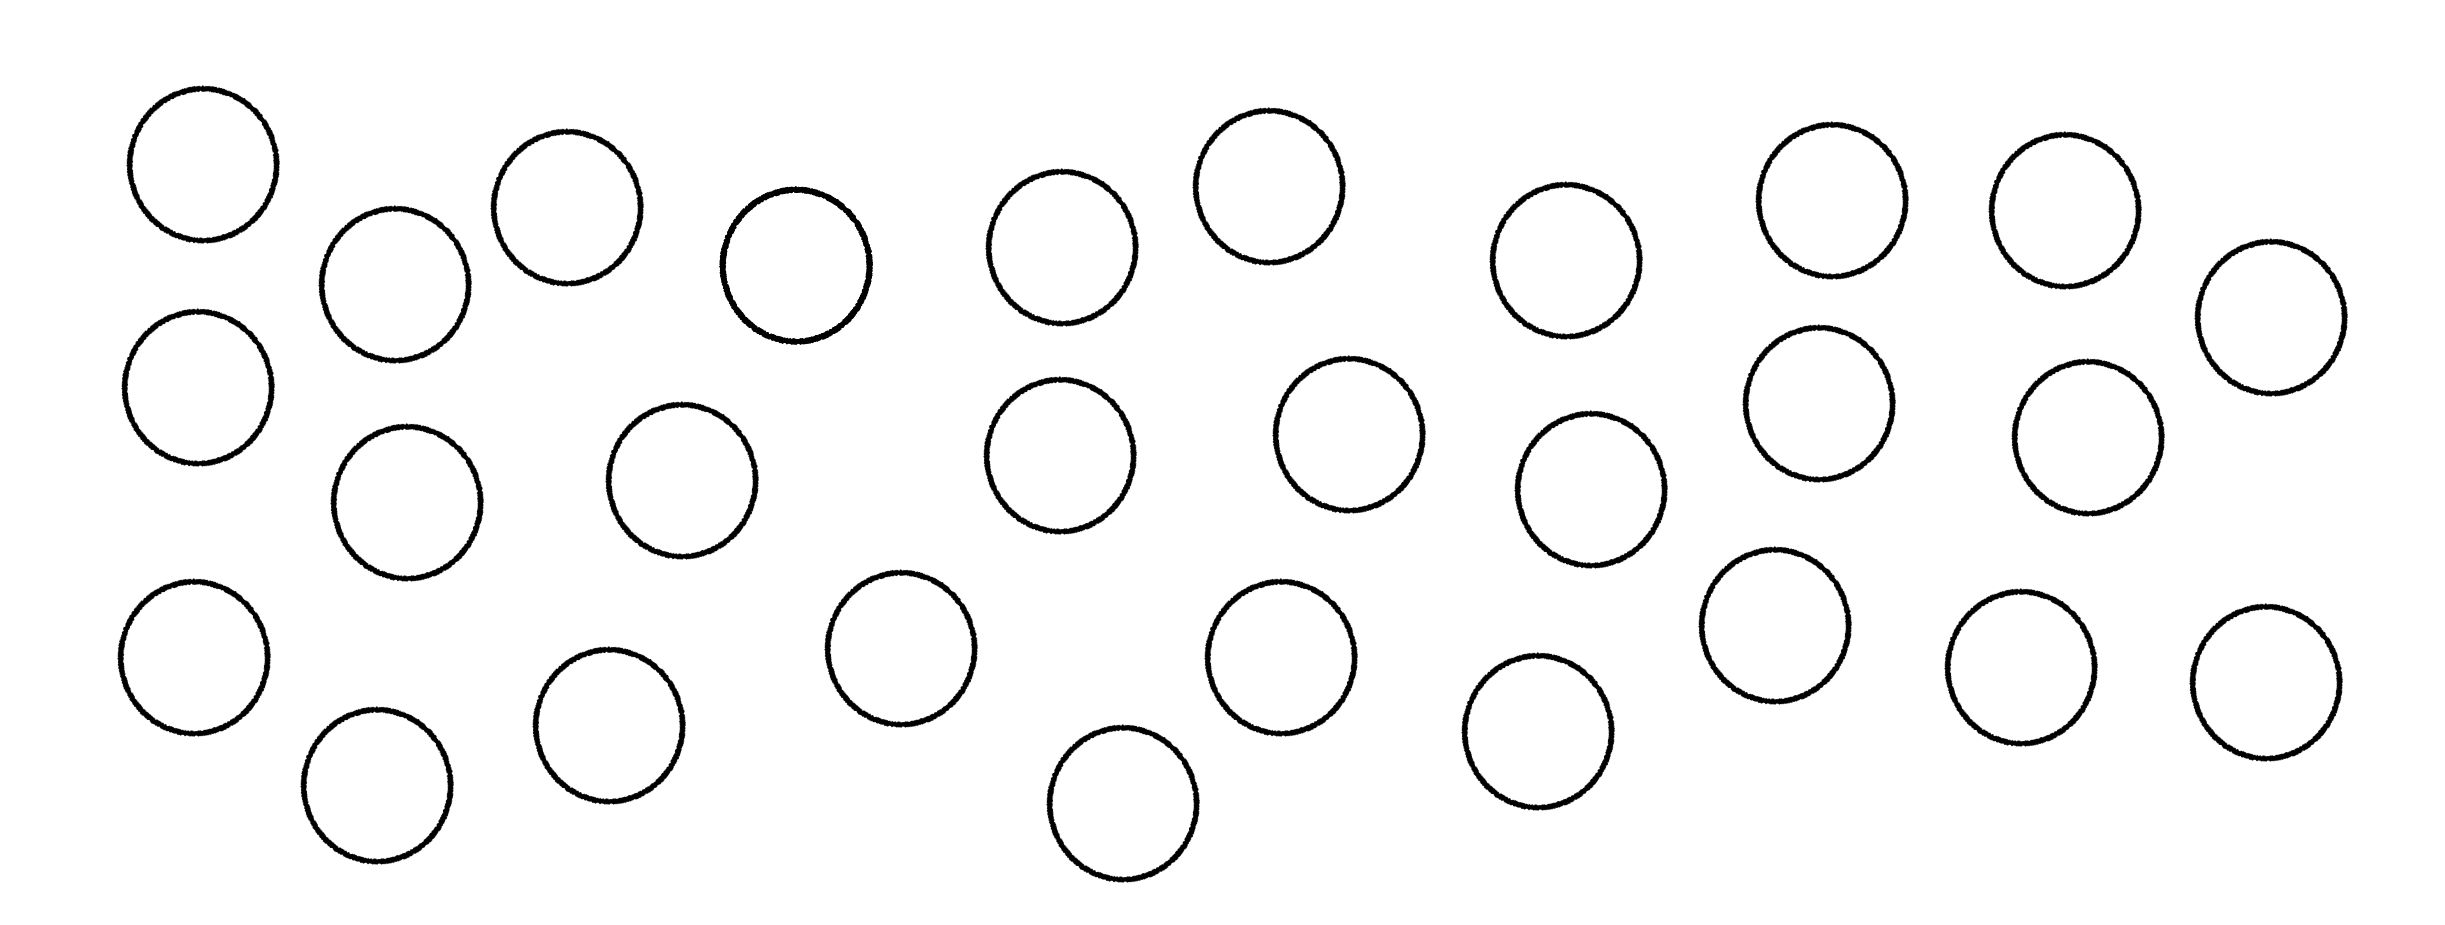
\includegraphics[width=\textheight ,
%    keepaspectratio]{surfacet1.jpg}}{test.mp4}

% \end{frame}
%%%%%%%%%%%%%%%%%%%%%%%%%%%%%%%%%%%%%%%%%%%%%%%%%%%%%%%%%%%%%%%%%%%

%%%%%%%%%%%%%%%%%%%%%%%%%%%%%%%%%%%%%%%%%%%%%%%%%%%%%%%%%%%%%%%%%%%
\newcounter{example}
 \setcounter{example}{1} 


 %%%%%%%%%%%%%%%%%%%%%%%%%%%%%%%%%%%%%%%%%%%%%%%%%%%%%%%%%%%%%%%



 \begin{frame}
  \frametitle{Let us calculate the wavelength of a laser}

  \textcolor{mypink1}{Position of dark fringes in a single slit of width $a$}
  \begin{figure}[h!]
    \begin{center}
      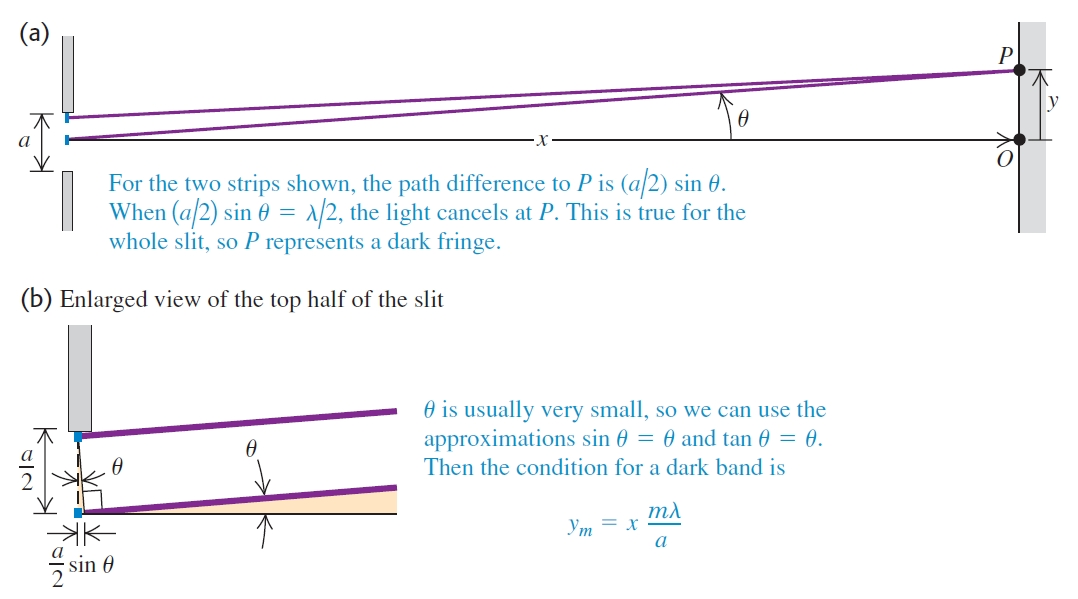
\includegraphics[height=2.5in]{images/1.jpg}
    \end{center}
  \end{figure}
\end{frame}
  
 %%%%%%%%%%%%%%%%%%%%%%%%%%%%%%%%%%%%%%%%%%%%%%%%%%%%%%%%%%%%%%%



 \begin{frame}
    \frametitle{Then...}
  
    \textcolor{mypink1}{Then...}
    \vspace{10mm}

    \begin{figure}[h!]
      \begin{center}
        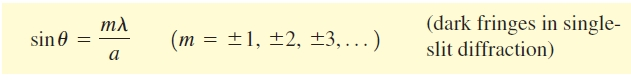
\includegraphics[height=0.5in]{images/2.jpg}
      \end{center}
    \end{figure}

    \pause
\vspace{5mm}
    for small angles:
    \vspace{5mm}


    \pause
\begin{equation*}
    \frac{y_m}{x}=\frac{m\lambda}{a}\pause\rightarrow y_m=x\frac{m\lambda}{a}
\end{equation*}



\end{frame}

 %%%%%%%%%%%%%%%%%%%%%%%%%%%%%%%%%%%%%%%%%%%%%%%%%%%%%%%%%%%%%%%



 \begin{frame}
    \frametitle{Intensity of the pattern}
  
    \textcolor{mypink1}{Position of dark fringes in a single slit of width $a$}
    \begin{figure}[h!]
      \begin{center}
        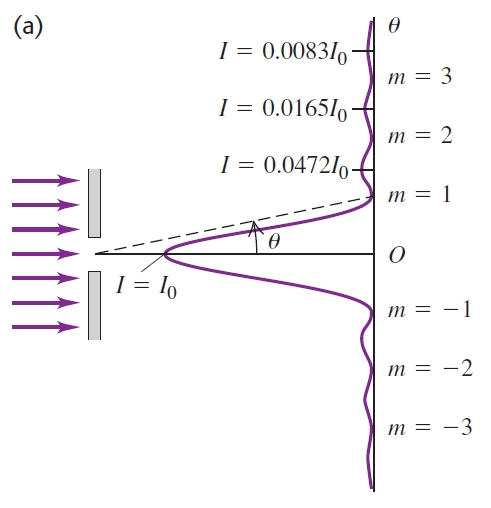
\includegraphics[height=2.5in]{images/3.jpg}
      \end{center}
    \end{figure}

  \end{frame}
    
   %%%%%%%%%%%%%%%%%%%%%%%%%%%%%%%%%%%%%%%%%%%%%%%%%%%%%%%%%%%%%%%

 %%%%%%%%%%%%%%%%%%%%%%%%%%%%%%%%%%%%%%%%%%%%%%%%%%%%%%%%%%%%%%%



 \begin{frame}
    \frametitle{What we observe is something like this}
  


\begin{columns}[c]
\column{2in}  % slides are 3in high by 5in wide

\textcolor{mypink1}{Position of dark fringes in a single slit of width $a$}
\begin{figure}[h!]
  \begin{center}
    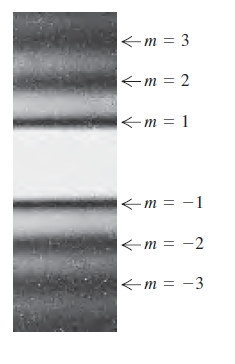
\includegraphics[height=2.5in]{images/4.jpg}
  \end{center}
\end{figure}


\column{2in}

\pause

Then, if we know  the position of the first dark fringe, the width of the slit and the 
distance to the screen, we can calculate $\lambda$ for a given source:
\vspace{5mm}

\pause
\begin{equation*}
    \lambda =\frac{ay_m}{xm}
\end{equation*}




\end{columns}



  \end{frame}
    
   %%%%%%%%%%%%%%%%%%%%%%%%%%%%%%%%%%%%%%%%%%%%%%%%%%%%%%%%%%%%%%%
   \begin{frame}
    \frametitle{What we observe is something like this}
  
If $a\sim 0.5$ mm, $y_m \sim 1$ cm, $x\sim 2.5$ m, $m=1$:\pause
\vspace{7mm}

\begin{equation*}
    \lambda \sim\frac{0.0005\times0.01}{2.5\times 1}\pause\sim 2\times 10^{-6}~m
\end{equation*}


  \end{frame}
    
   %%%%%%%%%%%%%%%%%%%%%%%%%%%%%%%%%%%%%%%%%%%%%%%%%%%%%%%%%%%%%%%


%%%%%%%%%%%%%%%%%%%%%%%%%%%%%%%%%%%%%%%%%%%%%%%%%%%%%%%%%%%%%%%
 \end{document}
%%%%%%%%%%%%%%%%%%%%%%%%%%%%%%%%%%%%%%%%%%%%%%%%%%%%%%%%%%%%%%%